% Chapter 2, Topic _Linear Algebra_ Jim Hefferon
%  http://joshua.smcvt.edu/linearalgebra
%  2001-Jun-11
\topic{Crystals}
\index{crystals|(}
Everyone has noticed that table salt\index{salt}
comes in little cubes.
\begin{center}
  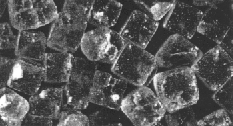
\includegraphics[height=1.25in]{vs/pix/salt.jpg} %1.25in tall
\end{center}
This orderly outside arises from an orderly inside\Dash 
the way the atoms lie is also cubical,
these cubes stack in neat rows and columns, and the salt faces
tend to be just an outer layer of cubes.
One cube of atoms is shown below.
Salt is sodium chloride and the
small spheres shown are sodium while the big ones are chloride.
To simplify the view, it only shows the sodiums and chlorides on the front, 
top, and right.
\begin{center}
  \includegraphics{vs/mp/ch2.1}
\end{center}
The specks of salt that we see above 
have many repetitions of this fundamental unit. 
A solid, such as table salt, 
with a regular internal structure is a \definend{crystal}.

We can restrict our attention to the front face.
There we have a square repeated many times giving a lattice of atoms.
\begin{center}
  \includegraphics{vs/mp/ch2.9}
\end{center}
The distance along the sides of each square 
cell is about $3.34$~\AA ngstroms
(an \AA ngstrom is $10^{-10}$~meters).
When we want to refer to atoms in the lattice 
that number is unwieldy, and 
so we 
take the square's side length as a unit.
That is, we naturally adopt this basis.
\begin{equation*}
  \sequence{\colvec{ 3.34 \\ 0},\colvec{0 \\ 3.34}}
\tag*{}\end{equation*}
Now we can describe, say, the atom in the upper right of the lattice
picture above
as $3\vec{\beta}_1+2\vec{\beta}_2$, instead of $10.02$~\AA ngstroms over
and $6.68$~up.

Another crystal from everyday experience is pencil lead.
It is \definend{graphite},\index{graphite} 
formed from carbon atoms arranged in this shape.
\begin{center}  %graphite
  \includegraphics{vs/mp/ch2.10}
\end{center}
This is a single plane of graphite, called \definend{graphene}.
A piece of graphite consists of many of these planes, layered.
The chemical bonds between the planes are
much weaker than the bonds inside the planes, which explains why 
pencils write\Dash the graphite can be sheared so that the planes slide 
off and are left on the paper.

We can get a convenient unit of length by
decomposing the hexagonal ring into three regions that are rotations
of this \definend{unit cell}.\index{crystals!unit cell} 
\begin{center}  %graphite
  \includegraphics{vs/mp/ch2.11}
\qquad\qquad
\includegraphics{vs/mp/ch2.12}
\end{center}
The vectors that form the sides of
that unit cell make a convenient basis.
The distance along the bottom  and slant is $1.42$~\AA ngstroms, 
so this
\begin{equation*}
  \sequence{\colvec{1.42 \\ 0}, \colvec{0.71 \\ 1.23}}
\tag*{}\end{equation*}   
is a good basis.

Another familiar crystal formed from carbon is diamond.\index{diamond}
Like table salt it is built from cubes but the structure inside each 
cube is more complicated. 
In addition to carbons at each corner,
\begin{center}
  \includegraphics{vs/mp/ch2.13}
\end{center}
there are carbons in the middle of each face. 
\begin{center}
  \includegraphics{vs/mp/ch2.14}
\end{center}
(To show the new face carbons clearly, 
the corner carbons are reduced to dots.)
There are also four more carbons inside the cube, 
two that are a quarter of the way up from the 
bottom and two that are a quarter of the way down from the top.
\begin{center}
  \includegraphics{vs/mp/ch2.15}  
\end{center}
(As before, carbons shown earlier are reduced here to dots.)
The distance along any edge of the cube is $2.18$~\AA ngstroms. 
Thus, a natural basis for describing the locations of the carbons
and the bonds between them, is this.
\begin{equation*}
  \sequence{\colvec{2.18 \\ 0 \\ 0}, 
            \colvec{0 \\ 2.18 \\ 0}, 
            \colvec{0 \\ 0 \\ 2.18}}
\tag*{}\end{equation*}   

The examples here show that
the structures of crystals is complicated enough to need
some organized system to give the locations of the atoms and how they
are chemically bound.
One tool for that organization is a convenient basis.
This application of bases is simple but it shows a 
science context where 
the idea arises naturally.
% The work in this chapter just takes this simple idea and develops it.

\begin{exercises}
  \item 
    How many fundamental regions are there in one face of a speck
    of salt? 
   (With a ruler, we can estimate that face is a square 
   that is $0.1$~cm on a side.)
   \begin{answer}
     Each fundamental unit is $3.34\times 10^{-10}$~cm, so there are
     about $0.1/(3.34\times 10^{-10})$ such units.
     That gives $2.99\times 10^{8}$, so there are something like
     $300,000,000$ (three hundred million) regions.     
   \end{answer}
  \item 
    In the graphite picture, imagine that we are interested in a point 
    $5.67$~\AA ngstroms over and $3.14$~\AA ngstroms up from the origin.
    \begin{exparts}
      \partsitem Express that point in terms of the basis given
        for graphite.
      \partsitem How many hexagonal shapes away is this point from the origin? 
      \partsitem Express that point in terms of a second basis,
        where the first basis vector is the same, but the second is 
        perpendicular to the first (going up the plane) and of the same length.
    \end{exparts} 
    \begin{answer}
      \begin{exparts}
        \partsitem We solve
          \begin{equation*}
            c_1\colvec{1.42 \\ 0}+c_2\colvec{0.71 \\ 1.23}
              =\colvec{5.67 \\ 3.14}
            \quad\implies\quad
            \begin{linsys}{2}
              1.42c_1  &+  &0.71c_2  &=  &5.67  \\
                       &   &1.23c_2  &=  &3.14
            \end{linsys}
          \tag*{}\end{equation*}
          to get $c_1\approx 2.74$ and $c_2\approx 2.55$.
        \partsitem Here is the point located in the lattice.
          In the picture on the left, superimposed on the unit cell are the
          two basis vectors $\vec{\beta}_1$ and $\vec{\beta}_2$, 
          and a box showing the offset of 
          $2.55\vec{\beta}_1+2.72\vec{\beta}_2$. 
          The picture on the right shows where that appears inside of 
          the crystal lattice, taking as the origin
          the lower left corner of the hexagon in the lower left. 
          \begin{center}  %graphite
            \includegraphics{vs/mp/ch2.17}
            \qquad
            \includegraphics{vs/mp/ch2.18}
       \end{center}
       So this point is two columns of hexagons over and  
       one hexagon up.
      \partsitem This second basis
          \begin{equation*}
            \sequence{\colvec{1.42 \\ 0},\colvec{0 \\ 1.42}}
          \tag*{}\end{equation*}
          makes the computation easier
          \begin{equation*}
            c_1\colvec{1.42 \\ 0}+c_2\colvec{0 \\ 1.42}
              =\colvec{5.67 \\ 3.14}
            \quad\implies\quad
            \begin{linsys}{2}
              1.42c_1  &   &         &=  &5.67  \\
                       &   &1.42c_2  &=  &3.14
            \end{linsys}
          \tag*{}\end{equation*}
          (we get $c_2\approx 2.21$ and $c_1\approx 3.99$), but it doesn't 
          seem to have to do much with the physical structure that we are
          studying. 
      \end{exparts}
    \end{answer}
  \item 
    Give the locations of the atoms in the diamond cube both
    in terms of the basis, and in \AA ngstroms.
    \begin{answer}
      In terms of the basis the locations of the corner atoms are
      $(0,0,0)$, $(1,0,0)$, \ldots, $(1,1,1)$.
      The locations of the face atoms are $(0.5,0.5,1)$, $(1,0.5,0.5)$,
      $(0.5,1,0.5)$, $(0,0.5,0.5)$, $(0.5,0,0.5)$, and $(0.5,0.5,0)$.
      The locations of the atoms a quarter of the way down from the top
      are $(0.75,0.75,0.75)$ and $(0.25,0.25,0.25)$. 
      The atoms a quarter of the way up from the bottom
      are at $(0.75,0.25,0.25)$ and $(0.25,0.75,0.25)$. 
      Converting to \AA ngstroms is easy.
    \end{answer}
  \item 
    This illustrates how we could compute the 
    dimensions of a unit cell from the shape 
    in which a substance crystallizes 
    (\cite{Ebbing}, p.~462).
    \begin{exparts}
      \partsitem Recall that there are $6.022\times 10^{23}$ atoms in a mole
        (this is Avogadro's number).
        From that, and the fact that platinum has a mass of $195.08$ grams
        per mole, calculate the mass of each atom.
      \partsitem Platinum crystallizes in a face-centered cubic lattice
        with atoms at each lattice point,
        that is, it looks like the middle picture given above for 
        the diamond crystal.
        Find the number of platinum's per unit cell
        (hint:~sum the fractions of platinum's that are inside of a single 
        cell).
      \partsitem From that, find the mass of a unit cell.
      \partsitem Platinum crystal has a 
        density of $21.45$ grams per cubic centimeter.
        From this, and the mass of a unit cell, calculate the volume of a 
        unit cell.
      \partsitem Find the length of each edge.
      \partsitem Describe a natural three-dimensional basis.
    \end{exparts}
    \begin{answer}
      \begin{exparts}
        \partsitem $195.08/6.02\times 10^{23}=3.239\times 10^{-22}$
        \partsitem Each platinum atom in the middle of each face is 
          split between two cubes, so that is $6/2=3$ atoms so far.
          Each atom at a corner is split among eight cubes, so 
          that makes an additional $8/8=1$~atom, so the total is $4$.
        \partsitem $4\cdot 3.239\times 10^{-22}=1.296\times 10^{-21}$
        \partsitem $1.296\times 10^{-21}/21.45=6.042\times 10^{-23}$ cubic
           centimeters
        \partsitem $3.924\times 10^{-8}$ centimeters.
        \partsitem 
            $\sequence{\colvec{3.924\times 10^{-8} \\ 0 \\ 0},
                       \colvec{0 \\ 3.924\times 10^{-8} \\ 0},
                       \colvec{0 \\ 0 \\ 3.924\times 10^{-8}}}$
      \end{exparts}
    \end{answer}
\end{exercises}
\index{crystals|)}
\endinput
